% K字 引入：三点A,P,B共线，三角 α 同侧，证 △PAC ~ △BPD
\documentclass[tikz,border=4pt]{standalone}
\usepackage{ctex}
\usepackage{amsmath}
\usetikzlibrary{calc}
\begin{document}
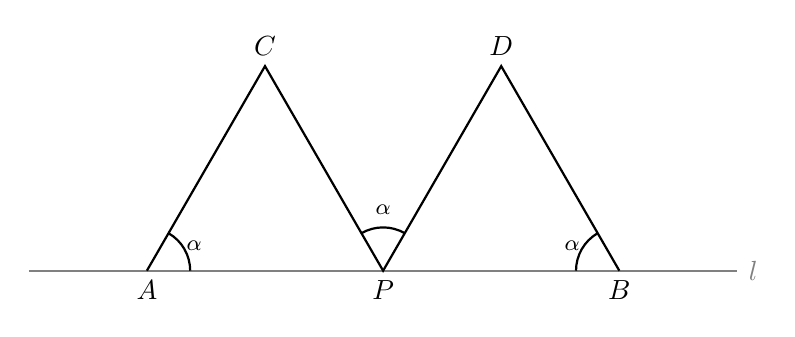
\begin{tikzpicture}[scale=1.0, thick]
  % α=60° K字
  \draw[gray] (-4.5,0)--(4.5,0);
  \node[gray] at (4.7,0) {$l$};
  \coordinate (A) at (-3,0);
  \coordinate (P) at (0,0);
  \coordinate (B) at (3,0);
  \coordinate (C) at (-1.5,2.598);
  \coordinate (D) at (1.5,2.598);
  \draw (A)--(C)--(P)--(D)--(B);
  \draw ($(A)+(0.55,0)$) arc[start angle=0, end angle=60, radius=0.55];
  \node at (-2.4,0.32) {\footnotesize $\alpha$};
  \draw ($(P)+({0.55*cos(60)},{0.55*sin(60)})$) arc[start angle=60, end angle=120, radius=0.55];
  \node at (0,0.78) {\footnotesize $\alpha$};
  \draw ($(B)+(-0.55,0)$) arc[start angle=180, end angle=120, radius=0.55];
  \node at (2.4,0.32) {\footnotesize $\alpha$};
  \node[below] at (A) {$A$};
  \node[below] at (P) {$P$};
  \node[below] at (B) {$B$};
  \node[above] at (C) {$C$};
  \node[above] at (D) {$D$};
\end{tikzpicture}
\end{document}
